\documentclass[conference]{IEEEtran}
\IEEEoverridecommandlockouts
\usepackage{cite}
\usepackage{amsmath,amssymb,amsfonts}
\usepackage{algorithmic}
\usepackage{algorithm}
\usepackage{graphicx}
\usepackage{textcomp}
\usepackage{xcolor}
\usepackage{tabularx}
\usepackage{tikz}
\usepackage{booktabs}
\usepackage{xurl}
\usetikzlibrary{shapes.geometric, arrows.meta, positioning, fit}

\def\BibTeX{{\rm B\kern-.05em{\sc i\kern-.025em b}\kern-.08em
    T\kern-.1667em\lower.7ex\hbox{E}\kern-.125emX}}
\begin{document}

\title{Attribution Without Validation: Measuring Downstream Bias\\
in Failure Attribution for Multi-Agent Text-to-SQL\\

}

\author{\IEEEauthorblockN{1\textsuperscript{st} Minh-Quang Nguyen}
\IEEEauthorblockA{\textit{Research Institute of Posts and Telecommunications} \\
\textit{Posts and Telecommunications Institute of Technology}\\
Hanoi, Vietnam \\
QuangNM.B23CC140@stu.ptit.edu.vn}
\and
\IEEEauthorblockN{2\textsuperscript{nd} Quang-Dai Tran}
\IEEEauthorblockA{\textit{Research Institute of Posts and Telecommunications} \\
\textit{Posts and Telecommunications Institute of Technology}\\
Hanoi, Vietnam \\
daitq@ptit.edu.vn}
}

\maketitle

\begin{abstract}
Recent advances in Large Language Models have improved Text-to-SQL performance and established Multi-Agent Systems (MAS) as a practical approach for strong end-to-end accuracy, yet current MAS pipelines behave as black boxes offering little visibility into failure origins. This work contributes a \emph{diagnostic framework}, a \emph{perturbation benchmark}, and---critically---a \emph{validation protocol for attribution heuristics themselves}. Central to the framework is a Logging Matrix recording 13 intermediate state variables across four pipeline stages (Intent, Schema, Skeleton, Execution), enabling automated failure localisation via backward state-differencing. Applied to $7{,}000$ Spider executions, the framework attributes $27.20\%$ of outcomes to structural skeleton defects while execution/syntax errors fall to $0.29\%$ after self-correction, a distribution that appears to show execution-centric repair is badly misdirected. We then subject the attribution heuristic to a test that prior work omits: evaluation against $398$ perturbation instances whose faulty stage is fixed by construction. The result is negative and unambiguous. Stage-level recall is $0\%$ for both injected intent faults and injected schema faults; instead, $60.5\%$ of all injected faults are absorbed into the \texttt{Skeleton} label and $38.8\%$ into \texttt{Execution}, in proportions essentially independent of where the fault was actually introduced. Backward state-differencing therefore exhibits a systematic \emph{downstream bias}: upstream semantic faults are masked by the structural mismatches they induce. Any stage distribution obtained this way must be reported as \emph{framework-attributed} rather than as an empirical property of the pipeline---a distinction the failure-attribution literature currently elides. We release the Logging Matrix, the perturbation benchmark, and the bias-measurement protocol so that attribution heuristics can be validated before their distributions are trusted.
\end{abstract}

\begin{IEEEkeywords}
Text-to-SQL, Multi-Agent Systems, Failure Attribution, Attribution Bias,
Diagnostic Benchmark, Negative Results, Large Language Models.
\end{IEEEkeywords}

\section{Introduction}
\subsection{Context}
Recent advances in LLMs have improved Text-to-SQL performance, with Multi-Agent Systems (MAS) decomposing the task into specialised agents---intent understanding, schema linking, skeleton generation, and execution---achieving strong results on benchmarks such as Spider and BIRD~\cite{yu_spider_2018}. However, high benchmark accuracy masks a critical limitation: MAS pipelines behave as black boxes, providing little visibility into \emph{who} (which agent) erred and \emph{when} (which stage) the error emerged~\cite{huo_bird-interact_2026, zhu_scot2s_2026}. This opacity impairs system design in several ways. Self-correction strategies remain largely blind, relying on execution-driven feedback that consumes excessive tokens while producing superficial fixes~\cite{zhu_scot2s_2026}. 

\subsection{Related works}
\label{sec:related}
Text-to-SQL research has evolved along several interconnected directions, from multi-agent task decomposition and error correction to failure attribution and diagnostic benchmarking; each contributing to, yet stopping short of, a unified framework for stage-level root-cause analysis.
\subsubsection{Multi-Agent Systems in Text-to-SQL}
Text-to-SQL has shifted from single-pass LLM generation to Multi-Agent Systems (MAS). DIN-SQL demonstrated that decomposing the task into schema linking, query classification, and self-correction yields roughly 10\% gains over monolithic prompting~\cite{pourreza_din-sql_2023}. Subsequent works further specialise agents for intent understanding, query planning, and SQL generation~\cite{chaturvedi2025sqlofthought, wang_mac-sql_2025, cen_sqlfixagent_2025}. Despite high execution accuracy on standard benchmarks, these systems remain end-to-end black boxes: intermediate states are not systematically logged, leaving it unclear which agent introduced an error~\cite{lei_spider_2025}.

\subsubsection{Error Analysis and Self-Correction}
Schema-linking mistakes and join-operation mismatches account for over 70\% of pipeline failures~\cite{shen_study_2025}, motivating various self-correction approaches. SCoT2S iteratively fixes errors at the SQL level~\cite{zhu_scot2s_2026}, EMLC applies multi-level correction across schema, skeleton, and executability layers~\cite{lei_emlc_2026}, and DAC decomposes correction into entity and skeleton sub-tasks~\cite{wang_dac_2025}. Despite these advances, most pipelines remain blind to root causes within the MAS architecture, patching final SQL without tracing which agent produced the original defect~\cite{shen_study_2025}.

\subsubsection{Automated Failure Attribution in LLM Multi-Agent Systems}
In~\cite{zhang2025which}, authors introduced the Who\&When dataset and showed that even the best attribution method achieves only 53.5\% accuracy in identifying responsible agents and 14.2\% in pinpointing failure steps. Our work differs in three respects: (1)~\emph{domain specificity}, targeting well-defined Text-to-SQL failure modes; (2)~\emph{structured intermediate logging} via a 13-variable Logging Matrix tailored to SQL generation semantics; and (3)~\emph{a perturbation benchmark with construction-time ground truth}, which lets the attribution heuristic be scored rather than assumed.

We read the 53.5\% figure of~\cite{zhang2025which} as the more important
result in that work, and our findings sharpen it. Their benchmark reports how
often attribution succeeds; ours reports what attribution does when it fails,
and the answer is not random error but a consistent directional bias toward
downstream stages. An attribution method can therefore be substantially worse
than its headline accuracy suggests, because its errors concentrate in a way
that manufactures an apparent bottleneck. We are not aware of prior work in
the Text-to-SQL setting that measures this directly, and we suggest the
omission is systemic: attribution heuristics are typically validated against
labels produced by inspecting the same intermediate signals the heuristic
consumes, which cannot expose a shared bias.

\subsubsection{Diagnostic Benchmarks and Robustness}
Standard benchmarks such as Spider~\cite{yu_spider_2018} emphasise Execution Accuracy and Exact Match, providing no signal about pipeline failure origins. Robustness-oriented works---including Dr.~Spider's 17 perturbation types~\cite{chang_drspider_2022}, Solid-SQL~\cite{liu_solid-sql_2025}, and SQL2NL~\cite{safarzadeh_evaluating_2025}---expose model brittleness but do not trace failures to specific pipeline stages. Our work extends these efforts by combining targeted perturbations with the Logging Matrix, enabling the first Text-to-SQL benchmark with explicit stage-level and agent-level root-cause annotations.

Without intermediate state logs, agent-level reasoning hallucinations cannot be systematically quantified~\cite{shen_select-sql_2024}. Finally, evaluation protocols focused solely on execution accuracy fail to provide the diagnostic signal needed for robust, trustworthy systems~\cite{huo_bird-interact_2026}.
\subsection{Objectives and contributions}
To address this gap, we introduce three complementary contributions. \textbf{First}, a \emph{Logging Matrix} that records 13 intermediate artifacts per agent, including parsed intent, filtered schema candidates, SQL skeleton with token-level provenance, and execution traces, enabling systematic comparison across pipeline states to localise discrepancies and hypothesise root causes. \textbf{Second}, a \emph{perturbation benchmark} of 400 instances constructed so that the faulty stage is known by design---schema-proxy substitutions targeting the schema-linking stage, and synonym paraphrases targeting intent understanding---providing ground truth against which an attribution heuristic can be scored. \textbf{Third}, and most consequential, a \emph{bias-measurement protocol} that turns this benchmark on the heuristic itself. Applying it to our own backward state-differencing procedure yields a negative result we report in full: stage-level recall is $0\%$ on both perturbation families, and injected faults are absorbed downstream in proportions nearly independent of their true origin. We argue this measurement should precede any published stage distribution, and that distributions reported without it---including the one in this paper's Table~\ref{tab:failures}---are properly described as \emph{framework-attributed} rather than as pipeline properties.

Throughout, we use \emph{Execution Accuracy} (EX)---whether the predicted query's result set matches that of the gold query---and \emph{Exact Match} (EM)---whether the predicted query matches the gold query structurally---following the definitions of Yu et al.~\cite{yu_spider_2018}.

The remainder of this paper is organized as follows. Section~\ref{sec:methodology} presents the methodology and section~\ref{sec:experiments} describes the diagnostic benchmark construction, experimental setup, and results. Finally, section~\ref{sec:conclusion} concludes the paper and discusses future work.



\section{Methodology}
\label{sec:methodology}

\subsection{Pipeline Breakdown}
Figure~\ref{fig:running_example} presents the proposed modular Text-to-SQL pipeline, per-stage error taxonomy, and Logging Matrix for automatic root-cause attribution. Following common practice~\cite{shen_study_2025}, the pipeline decomposes into four stages: intent understanding, schema selection, skeleton construction, and execution; each handled by a dedicated agent to reduce cognitive load and facilitate failure isolation.

\begin{figure}[htbp]
    \centering
    \resizebox{\columnwidth}{!}{
        % running_example.tex — Figure 1
% Included from conference_101719.tex via % running_example.tex — Figure 1
% Included from conference_101719.tex via % running_example.tex — Figure 1
% Included from conference_101719.tex via \input{running_example}
% Requires: \usetikzlibrary{shapes.geometric, arrows.meta, positioning}
%
% Illustrates the downstream-bias mechanism: a fault injected at the Intent
% stage propagates forward and is attributed to the Skeleton stage, because
% backward state-differencing meets the symptom before the cause.

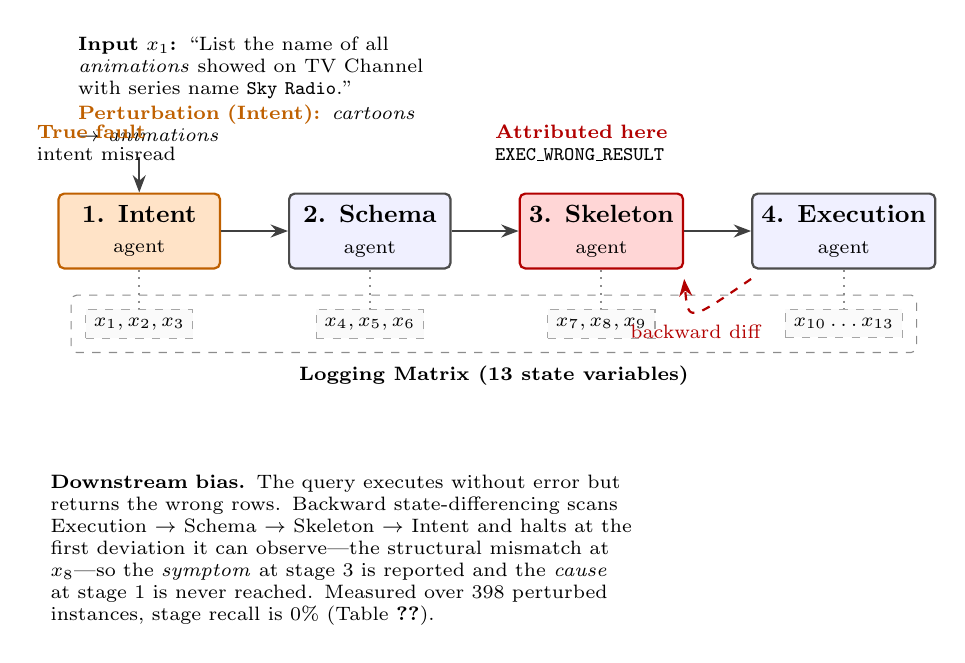
\begin{tikzpicture}[
  font=\small,
  stage/.style   = {rectangle, rounded corners=2pt, draw=black!70, thick,
                    minimum width=2.05cm, minimum height=0.95cm,
                    align=center, fill=blue!6},
  faulty/.style  = {stage, fill=orange!22, draw=orange!75!black},
  blamed/.style  = {stage, fill=red!16, draw=red!70!black},
  logbox/.style  = {rectangle, draw=black!35, dashed, inner sep=3pt,
                    align=center, font=\scriptsize, fill=black!2},
  note/.style    = {align=left, font=\scriptsize, text width=3.5cm},
  fwd/.style     = {-{Stealth[length=2.2mm]}, thick, black!75},
  back/.style    = {-{Stealth[length=2.2mm]}, thick, red!70!black, dashed}
]

% ---------- input ----------
\node[note, text width=4.4cm, anchor=west] (q) at (0,3.15)
  {\textbf{Input $x_1$:} ``List the name of all \emph{animations}
   showed on TV Channel with series name \texttt{Sky Radio}.''\\[1pt]
   \textcolor{orange!75!black}{\textbf{Perturbation (Intent):}}
   \emph{cartoons} $\rightarrow$ \emph{animations}};

% ---------- pipeline stages ----------
\node[faulty] (intent)   at (0.9,1.35) {\textbf{1. Intent}\\\scriptsize agent};
\node[stage, right=0.85cm of intent]  (schema)   {\textbf{2. Schema}\\\scriptsize agent};
\node[blamed, right=0.85cm of schema] (skeleton) {\textbf{3. Skeleton}\\\scriptsize agent};
\node[stage, right=0.85cm of skeleton](exec)     {\textbf{4. Execution}\\\scriptsize agent};

\draw[fwd] (intent)   -- (schema);
\draw[fwd] (schema)   -- (skeleton);
\draw[fwd] (skeleton) -- (exec);
\draw[fwd] ([yshift=-2pt]q.south -| intent.north) -- (intent.north);

% ---------- logging matrix ----------
\node[logbox, below=0.5cm of intent]   (l1) {$x_1,x_2,x_3$};
\node[logbox, below=0.5cm of schema]   (l2) {$x_4,x_5,x_6$};
\node[logbox, below=0.5cm of skeleton] (l3) {$x_7,x_8,x_9$};
\node[logbox, below=0.5cm of exec]     (l4) {$x_{10}\ldots x_{13}$};

\foreach \s/\l in {intent/l1, schema/l2, skeleton/l3, exec/l4}
  \draw[black!45, dotted, thick] (\s) -- (\l);

\node[draw=black!45, dashed, rounded corners=2pt, inner sep=5pt,
      fit=(l1)(l4), label={[font=\scriptsize\bfseries, yshift=-1pt]below:%
      Logging Matrix (13 state variables)}] (matrix) {};

% ---------- fault propagation ----------
\node[note, text width=2.6cm, anchor=south, font=\scriptsize]
  at ([yshift=0.28cm]intent.north)
  {\textcolor{orange!75!black}{\textbf{True fault}}\\ intent misread};

\node[note, text width=2.7cm, anchor=south, font=\scriptsize]
  at ([yshift=0.28cm]skeleton.north)
  {\textcolor{red!70!black}{\textbf{Attributed here}}\\ \texttt{EXEC\_WRONG\_RESULT}};

% ---------- backward diffing ----------
\draw[back] ([yshift=-0.12cm]exec.south west) .. controls +(-0.8,-0.55) ..
            ([yshift=-0.12cm]skeleton.south east)
  node[midway, below, font=\scriptsize, text=red!70!black, yshift=-1pt]
  {backward diff};

\node[note, text width=7.6cm, anchor=north west, font=\scriptsize]
  at (-0.35,-1.62)
  {\textbf{Downstream bias.} The query executes without error but returns the
   wrong rows. Backward state-differencing scans Execution $\rightarrow$
   Schema $\rightarrow$ Skeleton $\rightarrow$ Intent and halts at the first
   deviation it can observe---the structural mismatch at $x_8$---so the
   \emph{symptom} at stage~3 is reported and the \emph{cause} at stage~1 is
   never reached. Measured over 398 perturbed instances, stage recall is
   $0\%$ (Table~\ref{tab:confusion}).};

\end{tikzpicture}

% Requires: \usetikzlibrary{shapes.geometric, arrows.meta, positioning}
%
% Illustrates the downstream-bias mechanism: a fault injected at the Intent
% stage propagates forward and is attributed to the Skeleton stage, because
% backward state-differencing meets the symptom before the cause.

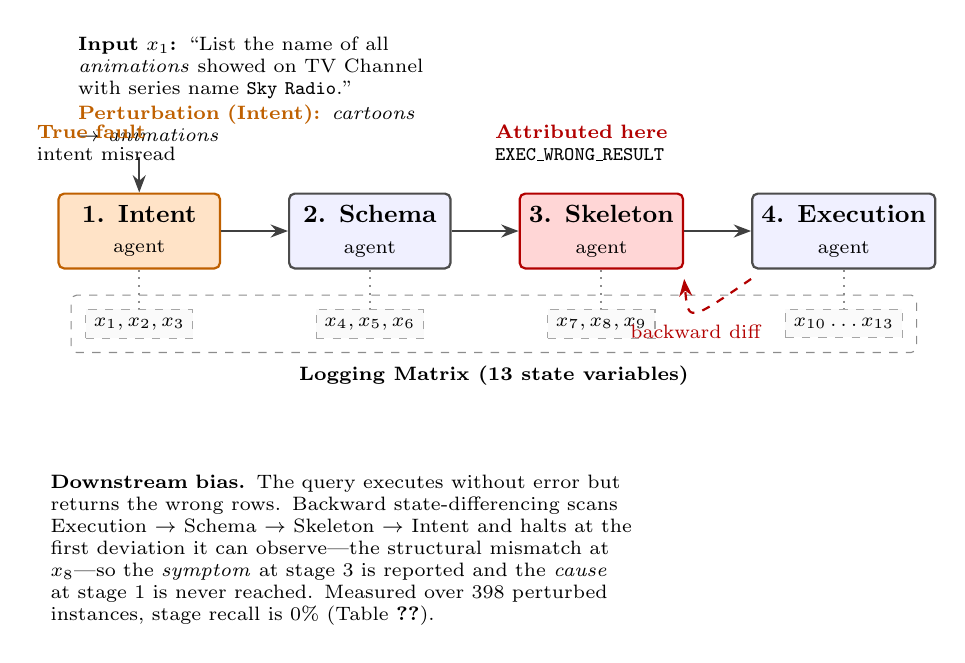
\begin{tikzpicture}[
  font=\small,
  stage/.style   = {rectangle, rounded corners=2pt, draw=black!70, thick,
                    minimum width=2.05cm, minimum height=0.95cm,
                    align=center, fill=blue!6},
  faulty/.style  = {stage, fill=orange!22, draw=orange!75!black},
  blamed/.style  = {stage, fill=red!16, draw=red!70!black},
  logbox/.style  = {rectangle, draw=black!35, dashed, inner sep=3pt,
                    align=center, font=\scriptsize, fill=black!2},
  note/.style    = {align=left, font=\scriptsize, text width=3.5cm},
  fwd/.style     = {-{Stealth[length=2.2mm]}, thick, black!75},
  back/.style    = {-{Stealth[length=2.2mm]}, thick, red!70!black, dashed}
]

% ---------- input ----------
\node[note, text width=4.4cm, anchor=west] (q) at (0,3.15)
  {\textbf{Input $x_1$:} ``List the name of all \emph{animations}
   showed on TV Channel with series name \texttt{Sky Radio}.''\\[1pt]
   \textcolor{orange!75!black}{\textbf{Perturbation (Intent):}}
   \emph{cartoons} $\rightarrow$ \emph{animations}};

% ---------- pipeline stages ----------
\node[faulty] (intent)   at (0.9,1.35) {\textbf{1. Intent}\\\scriptsize agent};
\node[stage, right=0.85cm of intent]  (schema)   {\textbf{2. Schema}\\\scriptsize agent};
\node[blamed, right=0.85cm of schema] (skeleton) {\textbf{3. Skeleton}\\\scriptsize agent};
\node[stage, right=0.85cm of skeleton](exec)     {\textbf{4. Execution}\\\scriptsize agent};

\draw[fwd] (intent)   -- (schema);
\draw[fwd] (schema)   -- (skeleton);
\draw[fwd] (skeleton) -- (exec);
\draw[fwd] ([yshift=-2pt]q.south -| intent.north) -- (intent.north);

% ---------- logging matrix ----------
\node[logbox, below=0.5cm of intent]   (l1) {$x_1,x_2,x_3$};
\node[logbox, below=0.5cm of schema]   (l2) {$x_4,x_5,x_6$};
\node[logbox, below=0.5cm of skeleton] (l3) {$x_7,x_8,x_9$};
\node[logbox, below=0.5cm of exec]     (l4) {$x_{10}\ldots x_{13}$};

\foreach \s/\l in {intent/l1, schema/l2, skeleton/l3, exec/l4}
  \draw[black!45, dotted, thick] (\s) -- (\l);

\node[draw=black!45, dashed, rounded corners=2pt, inner sep=5pt,
      fit=(l1)(l4), label={[font=\scriptsize\bfseries, yshift=-1pt]below:%
      Logging Matrix (13 state variables)}] (matrix) {};

% ---------- fault propagation ----------
\node[note, text width=2.6cm, anchor=south, font=\scriptsize]
  at ([yshift=0.28cm]intent.north)
  {\textcolor{orange!75!black}{\textbf{True fault}}\\ intent misread};

\node[note, text width=2.7cm, anchor=south, font=\scriptsize]
  at ([yshift=0.28cm]skeleton.north)
  {\textcolor{red!70!black}{\textbf{Attributed here}}\\ \texttt{EXEC\_WRONG\_RESULT}};

% ---------- backward diffing ----------
\draw[back] ([yshift=-0.12cm]exec.south west) .. controls +(-0.8,-0.55) ..
            ([yshift=-0.12cm]skeleton.south east)
  node[midway, below, font=\scriptsize, text=red!70!black, yshift=-1pt]
  {backward diff};

\node[note, text width=7.6cm, anchor=north west, font=\scriptsize]
  at (-0.35,-1.62)
  {\textbf{Downstream bias.} The query executes without error but returns the
   wrong rows. Backward state-differencing scans Execution $\rightarrow$
   Schema $\rightarrow$ Skeleton $\rightarrow$ Intent and halts at the first
   deviation it can observe---the structural mismatch at $x_8$---so the
   \emph{symptom} at stage~3 is reported and the \emph{cause} at stage~1 is
   never reached. Measured over 398 perturbed instances, stage recall is
   $0\%$ (Table~\ref{tab:confusion}).};

\end{tikzpicture}

% Requires: \usetikzlibrary{shapes.geometric, arrows.meta, positioning}
%
% Illustrates the downstream-bias mechanism: a fault injected at the Intent
% stage propagates forward and is attributed to the Skeleton stage, because
% backward state-differencing meets the symptom before the cause.

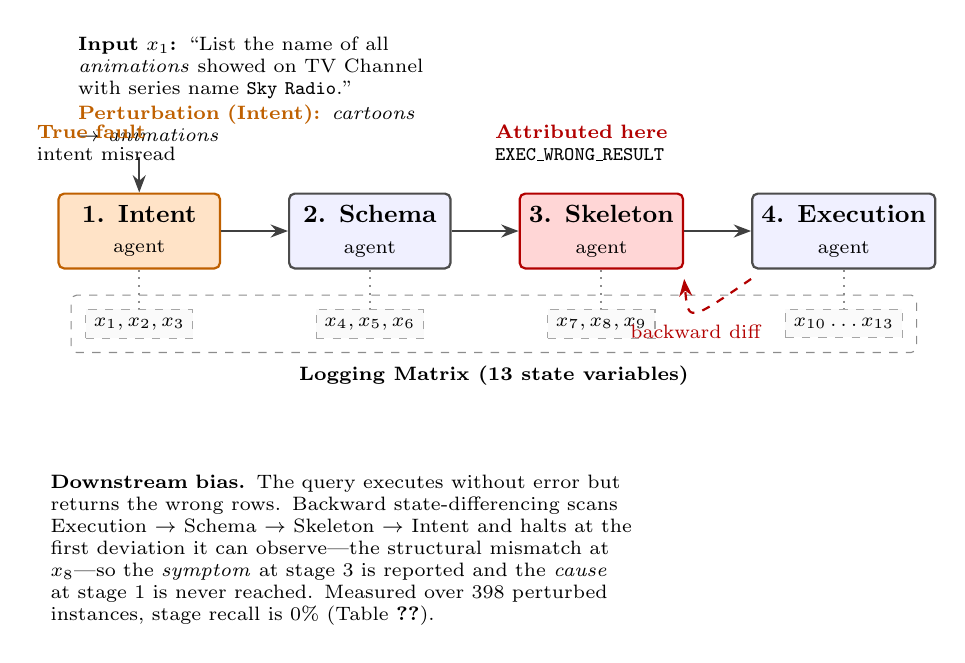
\begin{tikzpicture}[
  font=\small,
  stage/.style   = {rectangle, rounded corners=2pt, draw=black!70, thick,
                    minimum width=2.05cm, minimum height=0.95cm,
                    align=center, fill=blue!6},
  faulty/.style  = {stage, fill=orange!22, draw=orange!75!black},
  blamed/.style  = {stage, fill=red!16, draw=red!70!black},
  logbox/.style  = {rectangle, draw=black!35, dashed, inner sep=3pt,
                    align=center, font=\scriptsize, fill=black!2},
  note/.style    = {align=left, font=\scriptsize, text width=3.5cm},
  fwd/.style     = {-{Stealth[length=2.2mm]}, thick, black!75},
  back/.style    = {-{Stealth[length=2.2mm]}, thick, red!70!black, dashed}
]

% ---------- input ----------
\node[note, text width=4.4cm, anchor=west] (q) at (0,3.15)
  {\textbf{Input $x_1$:} ``List the name of all \emph{animations}
   showed on TV Channel with series name \texttt{Sky Radio}.''\\[1pt]
   \textcolor{orange!75!black}{\textbf{Perturbation (Intent):}}
   \emph{cartoons} $\rightarrow$ \emph{animations}};

% ---------- pipeline stages ----------
\node[faulty] (intent)   at (0.9,1.35) {\textbf{1. Intent}\\\scriptsize agent};
\node[stage, right=0.85cm of intent]  (schema)   {\textbf{2. Schema}\\\scriptsize agent};
\node[blamed, right=0.85cm of schema] (skeleton) {\textbf{3. Skeleton}\\\scriptsize agent};
\node[stage, right=0.85cm of skeleton](exec)     {\textbf{4. Execution}\\\scriptsize agent};

\draw[fwd] (intent)   -- (schema);
\draw[fwd] (schema)   -- (skeleton);
\draw[fwd] (skeleton) -- (exec);
\draw[fwd] ([yshift=-2pt]q.south -| intent.north) -- (intent.north);

% ---------- logging matrix ----------
\node[logbox, below=0.5cm of intent]   (l1) {$x_1,x_2,x_3$};
\node[logbox, below=0.5cm of schema]   (l2) {$x_4,x_5,x_6$};
\node[logbox, below=0.5cm of skeleton] (l3) {$x_7,x_8,x_9$};
\node[logbox, below=0.5cm of exec]     (l4) {$x_{10}\ldots x_{13}$};

\foreach \s/\l in {intent/l1, schema/l2, skeleton/l3, exec/l4}
  \draw[black!45, dotted, thick] (\s) -- (\l);

\node[draw=black!45, dashed, rounded corners=2pt, inner sep=5pt,
      fit=(l1)(l4), label={[font=\scriptsize\bfseries, yshift=-1pt]below:%
      Logging Matrix (13 state variables)}] (matrix) {};

% ---------- fault propagation ----------
\node[note, text width=2.6cm, anchor=south, font=\scriptsize]
  at ([yshift=0.28cm]intent.north)
  {\textcolor{orange!75!black}{\textbf{True fault}}\\ intent misread};

\node[note, text width=2.7cm, anchor=south, font=\scriptsize]
  at ([yshift=0.28cm]skeleton.north)
  {\textcolor{red!70!black}{\textbf{Attributed here}}\\ \texttt{EXEC\_WRONG\_RESULT}};

% ---------- backward diffing ----------
\draw[back] ([yshift=-0.12cm]exec.south west) .. controls +(-0.8,-0.55) ..
            ([yshift=-0.12cm]skeleton.south east)
  node[midway, below, font=\scriptsize, text=red!70!black, yshift=-1pt]
  {backward diff};

\node[note, text width=7.6cm, anchor=north west, font=\scriptsize]
  at (-0.35,-1.62)
  {\textbf{Downstream bias.} The query executes without error but returns the
   wrong rows. Backward state-differencing scans Execution $\rightarrow$
   Schema $\rightarrow$ Skeleton $\rightarrow$ Intent and halts at the first
   deviation it can observe---the structural mismatch at $x_8$---so the
   \emph{symptom} at stage~3 is reported and the \emph{cause} at stage~1 is
   never reached. Measured over 398 perturbed instances, stage recall is
   $0\%$ (Table~\ref{tab:confusion}).};

\end{tikzpicture}

    }
    \caption{The downstream-bias mechanism. A fault injected at the Intent
    stage (orange) propagates forward and produces a syntactically valid
    query that returns the wrong rows. Because backward state-differencing
    scans from Execution upstream and halts at the first observable
    deviation, the Failure Attribution Framework reports the Skeleton stage
    (red)---the symptom---and never reaches the cause. All four stages are
    logged; the Intent stage is nonetheless never blamed.}
    \label{fig:running_example}
\end{figure}


\subsubsection{Step 1: Intent (Understanding the Question)}
The first stage interprets the natural-language question and extracts the
underlying semantic intent. The agent parses the input to identify entities,
filter conditions, required aggregations (e.g., count, sum, max/min), and
temporal or spatial constraints. The output is an abstract, semantic
representation of the user's information need rather than a concrete SQL
statement~\cite{shen_study_2025}.

\subsubsection{Step 2: Schema (Schema Filtering)}
The schema stage narrows the search space over the database. Given the
intent from Step 1, the agent maps linguistic cues to schema elements and
selects only those tables and columns necessary to answer the question. The
output is a reduced, filtered schema that removes noisy elements and keeps
only the relevant structure~\cite{yang_sql--schema_2024}.

\subsubsection{Step 3: Skeleton (SQL Skeleton Construction)}
The third stage builds the logical structure of the SQL query. Using the
filtered schema from Step 2, the agent arranges core clauses such as
\texttt{SELECT}, \texttt{FROM}, \texttt{JOIN}, \texttt{WHERE},
\texttt{GROUP BY}, and \texttt{ORDER BY}. Concrete values may be left as
placeholders (e.g., \texttt{\_} or \texttt{?}), so the output is a
syntactically structured SQL template or skeleton~\cite{lei_emlc_2026}.

\subsubsection{Step 4: Execution (Finalization and Execution)}
The final stage completes the SQL and runs it against the database. The
agent fills in specific values into the skeleton, producing a fully
executable SQL statement, and sends it to the DBMS. The output is either a
result set or an error message from the DB engine~\cite{yu_spider_2018}.

\subsection{Error Taxonomy: Per-Stage Failure Types}
When a Text-to-SQL pipeline returns an incorrect result, the root cause
usually lies in one of the four steps above. Our error taxonomy categorises
mistakes according to the stage where the fault first appears, enabling
attribution at the agent level~\cite{shen_study_2025}.

\subsubsection{Errors at Step 1: Intent (Misunderstanding)}
\begin{itemize}
  \item \textbf{Missing Condition:} The model neglects an important clause
  present in the natural-language question (e.g., ignoring the temporal
  constraint ``2023'').
  \item \textbf{Misinterpretation:} The model misreads the mathematical or
  logical operator (e.g., computing a sum when an average is requested)~\cite{shen_study_2025}.
\end{itemize}

\subsubsection{Errors at Step 2: Schema (Schema Selection Errors)}
\begin{itemize}
  \item \textbf{Missing Schema:} The model fails to include a table or column
  essential for the query, leading to missing data or invalid join
  paths~\cite{chang_drspider_2022}.
  \item \textbf{Redundant Schema (Hallucination):} The model selects extra
  tables or references columns that do not exist, often inducing unintended
  Cartesian products~\cite{lei_emlc_2026}.
\end{itemize}

\subsubsection{Errors at Step 3: Skeleton (Structural / Logical Errors)}
\begin{itemize}
  \item \textbf{Wrong JOIN Logic:} Incorrect join path, join type, or
  \texttt{ON} condition.
  \item \textbf{Wrong Aggregation / Grouping:} Wrong aggregation function or
  incorrect \texttt{GROUP BY} column~\cite{shen_study_2025}.
  \item \textbf{Nesting / Subquery Errors:} Misstructured subqueries or set
  operations (e.g., \texttt{INTERSECT},
  \texttt{EXCEPT})~\cite{chen_text--sql_2023}.
\end{itemize}

\subsubsection{Errors at Step 4: Execution (Execution / Syntax Errors)}
\begin{itemize}
  \item \textbf{Syntax Error:} SQL violates basic grammar rules (e.g.,
  missing parentheses)~\cite{lei_emlc_2026}.
  \item \textbf{Type Mismatch:} Values of incompatible types are compared.
  \item \textbf{Wrong / Empty Result:} Syntactically valid SQL that returns
  an incorrect or empty result due to silent semantic errors introduced in
  earlier stages~\cite{shen_study_2025}.
\end{itemize}

\subsection{The Logging Matrix Design}
To make failure patterns observable and attributable in a MAS, we design a
Logging Matrix that records the state of the pipeline at 13 key checkpoints.
Each pipeline run is stored as a \texttt{PipelineLogEntry}, a structured JSON
object. By logging intermediate representations $x_i$ and coupling them with
lightweight detection heuristics, we establish a comprehensive failure
attribution mechanism~\cite{zhang2025which}.

\subsubsection{State Variables to Log}
We define 13 signals $(x_1 \to x_{13})$ that correspond to the main stages
of our pipeline and its analysis modules, as summarised in
Table~\ref{tab:logging}. This set is sufficient for robust
root-cause localization and failure attribution across agents.

\begin{table}[htbp]
\centering
\caption{State Variables Logged in the Pipeline}
\begin{tabular}{lp{6.5cm}}
\toprule
Notation & Stage / Description \& Content to Log \\
\midrule
$x_1$  & \textbf{Input (Raw Query):} Natural-language question, \texttt{db\_id}, full schema, auxiliary metadata. \\
$x_2$  & \textbf{External Knowledge:} Domain hints and contextual constraints injected externally. \\
$x_3$  & \textbf{Clarified Intent:} Refined representation of user intent, subtasks, and detected conditions. \\
$x_4$  & \textbf{Full Schema:} Complete database schema (all tables and columns). \\
$x_5$  & \textbf{Filtered Schema:} Pruned schema subset; irrelevant tables/columns removed. \\
$x_6$  & \textbf{Schema Alignment:} Token-to-schema mapping with confidence scores. \\
$x_7$  & \textbf{Query Plan:} Logical plan describing required joins, aggregations, and reasoning trace. \\
$x_8$  & \textbf{SQL Skeleton:} Structured SQL template with clause-level placeholders. \\
$x_9$  & \textbf{Candidate SQLs:} Multiple candidate SQL statements before final selection. \\
$x_{10}$ & \textbf{Execution (SQL):} Final executable SQL passed to the DBMS. \\
$x_{11}$ & \textbf{Execution (Result):} Result set on success, or error message / traceback on failure. \\
$x_{12}$ & \textbf{Failure Analysis:} Structured record with root-cause label, explanation, and suggested correction. \\
$x_{13}$ & \textbf{Repaired SQL:} Corrected SQL generated from $x_{12}$ for re-execution. \\
\bottomrule
\end{tabular}
\label{tab:logging}
\end{table}

\subsubsection{Backward Diffing for Root-Cause Diagnosis}

To attribute a failure to a specific step, we apply a backward diffing
strategy that starts from the final outcome $x_{11}$ and compares backward
through each state $x_i$ until we detect the first significant deviation from
expected behaviour. Algorithm~\ref{alg:backdiff} provides the formal
procedure.

\begin{algorithm}
\caption{Backward Diffing for Root-Cause Attribution}
\label{alg:backdiff}
\begin{algorithmic}[1]
\REQUIRE Log entry $(x_1, \ldots, x_{13})$, gold SQL $q^*$
\ENSURE Root-cause label $L$
\IF{$x_{11}$ contains a DB engine error}
    \STATE $L \leftarrow \texttt{EXECUTION\_SYNTAX}$; \textbf{return}
\ENDIF
\IF{$\text{result}(x_{10}) \neq \text{result}(q^*)$}
    \IF{$x_5$ is missing tables/columns required by $q^*$}
        \STATE $L \leftarrow \texttt{SCHEMA\_MISSING}$; \textbf{return}
    \ENDIF
    \IF{$x_6$ maps tokens to non-existent schema elements}
        \STATE $L \leftarrow \texttt{SCHEMA\_HALLUCINATION}$; \textbf{return}
    \ENDIF
    \IF{clauses in $x_8$ are absent from $x_{10}$}
        \STATE $L \leftarrow \texttt{SKELETON\_STRUCTURAL}$; \textbf{return}
    \ENDIF
    \IF{$x_3$ omits conditions present in $x_1$}
        \STATE $L \leftarrow \texttt{INTENT\_MISSING\_CONDITION}$; \textbf{return}
    \ENDIF
\ENDIF
\STATE $L \leftarrow \texttt{UNKNOWN}$; \textbf{return}
\end{algorithmic}
\end{algorithm}

\noindent\textbf{Threshold justification.}

The ambiguity range $[0.30, 0.55]$ for schema alignment confidence ($x_6$) was determined empirically on 50 development-set queries: scores below $0.30$ indicate clear misalignment, above $0.55$ indicate confident alignment, and the intermediate band flags uncertain alignment between plausible column candidates. The full detection logic spans four steps:

\begin{itemize}
  \item \textbf{Step A: Intent Understanding} $(x_1, x_2, x_3)$. Low keyword-coverage flags missing conditions; constraints in $x_3$ absent from $x_1$ or $x_2$ flag hallucinated assumptions~\cite{ding_ambisql_2025}.
  \item \textbf{Step B: Schema Linking} $(x_4, x_5, x_6)$. Missing required tables or columns flag \texttt{SCHEMA\_MISSING}; mappings to non-existent elements flag \texttt{SCHEMA\_HALLUCINATION}; confidence in $[0.30, 0.55]$ flags uncertain alignment~\cite{yang_sql--schema_2024, zhu_scot2s_2026}.
  \item \textbf{Step C: SQL Generation} $(x_7, x_8, x_9)$. Missing \texttt{JOIN} or \texttt{GROUP BY} operations flag a \emph{plan--execution mismatch}; absent expected clauses flag \emph{skeleton missing clauses}; inconsistent candidates in $x_9$ are quantified as a self-consistency score~\cite{zhu_scot2s_2026, lei_emlc_2026}.
  \item \textbf{Step D: Execution and Verification} $(x_{10}, x_{11}, x_{12}, x_{13})$. Engine errors in $x_{10}$ propagate to $x_{12}$; silent semantic errors are assigned root-cause labels by combining $x_{11}$ with $x_{12}$; $x_{13}$ is compared with $x_9$ to detect repair regression.
\end{itemize}

\subsection{Ordering Sensitivity and Downstream Bias}
\label{sec:bias_design}

Algorithm~\ref{alg:backdiff} evaluates its conditions in a fixed
downstream-first order: execution, then schema, then skeleton, then intent.
This ordering is not incidental to the method---it is forced by the structure
of the pipeline. Only the execution stage produces an unambiguous, externally
verifiable signal (a DB engine error or a result-set mismatch); upstream
states are latent and can be judged only by proxy heuristics over $x_3$,
$x_5$, and $x_6$.

The ordering has a consequence that, to our knowledge, prior failure-attribution
work has not measured. Because a fault at any stage propagates forward, an
intent-stage fault almost always \emph{also} manifests as a structural
discrepancy at $x_8$ or a result mismatch at $x_{11}$. A downstream-first
procedure therefore encounters the symptom before it encounters the cause, and
returns the symptom. Formally, for a fault injected at stage $s$ with observed
label $\hat{L}$, the procedure yields $P(\hat{L} = s)$ that may be far below
$1$ even when the injected fault is the sole cause of failure, so the
attributed distribution $P(\hat{L})$ is not an estimator of the true fault
distribution $P(s)$.

Two further design choices compound this. First, the intent branch fires only
under narrow conditions---an explicit \texttt{is\_ambiguous} flag on $x_3$, or
a clarified question shorter than $60\%$ of the original. Neither triggers for
a fluent paraphrase that the intent agent confidently misreads, which is
precisely the failure mode of interest. Second, the schema branch requires a
gold-SQL table to be absent from $x_5$; a schema agent that selects a
\emph{plausible but wrong} table passes this test.

We therefore treat the attribution heuristic as an object of measurement rather
than as a trusted instrument, and report its behaviour in
Section~\ref{sec:bias_results}.

\section{Experiments and Results}
\label{sec:experiments}

\subsection{Benchmark Construction and Data Selection}
\label{sec:benchmark}

We adopt the Spider dataset~\cite{yu_spider_2018}, a large-scale cross-domain benchmark covering approximately 200 relational databases across 138 domains, with queries categorised into four difficulty levels (\textit{Easy}, \textit{Medium}, \textit{Hard}, \textit{Extra-Hard}) by structural complexity.

Two distinct data collections are used, and we state their relationship explicitly to avoid the ambiguity of a single aggregate count. \textbf{(i)~The distribution set}: all $7{,}000$ instances of the Spider \emph{training} split, executed end-to-end through the pipeline and used for the stage distribution in Section~\ref{sec:failure_dist}. \textbf{(ii)~The perturbation set}: $400$ instances drawn from the Spider \emph{validation} split and from Spider-Syn~\cite{gan_spider_syn_2021}, perturbed so that the faulty stage is fixed by construction, and used exclusively in Section~\ref{sec:bias_results} to score the attribution heuristic. The two sets are disjoint in purpose and are never pooled into a single accuracy figure. Table~\ref{tab:benchmark} summarises the perturbation set.

\begin{table}[htbp]
\centering
\caption{Diagnostic Benchmark Composition}
\begin{tabular}{llcc}
\toprule
Source & Perturbation & \# & Target stage \\
\midrule
Spider validation & Schema proxy      & 200 & Schema \\
Spider-Syn        & Intent paraphrase & 200 & Intent \\
\midrule
\multicolumn{2}{l}{\textbf{Total} (398 unique)} & \textbf{400} & -- \\
\bottomrule
\end{tabular}
\label{tab:benchmark}
\end{table}

Ground truth for this set is established \emph{by construction} rather than by
post-hoc annotation: a schema-proxy instance substitutes a distractor table
name that is lexically close to the gold table, so the schema-linking stage is
the stage placed under stress; an intent-paraphrase instance rewrites the
question using Spider-Syn synonym substitutions that preserve the gold SQL, so
the intent stage is the stage placed under stress. Two of the 400 items are
duplicate \texttt{(db\_id, question)} pairs, leaving 398 unique instances; all
reported rates use the 398 unique items.

We emphasise a methodological point that motivates the whole of
Section~\ref{sec:bias_results}. Construction-time ground truth is weaker than
human annotation in one respect---it certifies where the fault was
\emph{injected}, not that the pipeline actually failed there---but stronger in
another: it is not produced by the same reasoning process being evaluated, and
so cannot silently inherit that process's biases. An attribution heuristic
scored against labels derived from its own intermediate signals would be
scored against itself.

\subsection{Experimental Setup}

The experiments are conducted in a standardised Multi-Agent environment:

\begin{itemize}
  \item \textbf{LLM Backbone:} All pipeline executions are powered by
  GPT-4o. This model serves as the primary reasoning engine, responsible
  for intent parsing, schema filtering, and SQL skeleton construction.
  \item \textbf{Execution Environment:} Predicted SQL queries are executed
  against local SQLite databases to obtain deterministic execution feedback
  (syntax exceptions or result sets).
  \item \textbf{Logging and Configuration:} State variables are stored in a
  structured JSON format recording the exact provenance of data across the
  pipeline, from the input question and \texttt{difficulty} label to
  intermediate SQL generation and boolean execution flags.
\end{itemize}

\noindent\textbf{Note on pipeline EX rate.}
Our MAS pipeline achieves a $62.21\%$ end-to-end EX rate on the Spider train
set before rerun, improving to $70.10\%$ after self-correction (both computed
over the $6{,}782$ instances that completed without infrastructure failure;
see below). This is intentionally below published state-of-the-art EX figures
because our pipeline is designed as a \emph{diagnostic testbed} rather than a
performance-optimised system---the diagnostic value of the Logging Matrix
depends on failures being present to attribute.

\noindent\textbf{Note on Exact Match.}
We do not report EM. Our implementation compared normalised query strings for
literal equality, which is not the Exact Set Match of the official Spider
evaluator---the latter parses each query into clause-level components and
compares them as sets, disregarding clause order and literal values. Under
string equality the measured rate was $0.00\%$ across all $7{,}000$
instances, a figure that reflects the comparison procedure rather than the
model: semantically and structurally correct predictions are rejected for
differing in whitespace, quoting, or alias naming. Rather than report a
number produced by a non-standard evaluator, we omit the metric. Nothing in
this paper's argument depends on EM; the observation it was previously used
to support---that predictions are frequently semantically equivalent but
structurally divergent from gold---is established directly by the stage
analysis below.

\noindent\textbf{Treatment of infrastructure failures.}
Of the $7{,}000$ runs, $218$ terminated in API or network timeouts after
rerun ($464$ before rerun). These are properties of the execution environment,
not of the pipeline's reasoning, and a root-cause taxonomy over pipeline
stages has no defensible slot for them. We therefore exclude them from the
taxonomy and from all denominators, reporting stage rates over the
$6{,}782$ instances that completed ($6{,}536$ pre-rerun). Excluded counts are
reported separately in Table~\ref{tab:failures} so that the full $7{,}000$
remains reconcilable.

\subsection{Failure Distribution Analysis}
\label{sec:failure_dist}

Across the logged runs, the Logging Matrix assigns each outcome a stage label.
The resulting distribution before and after rerun is summarised in
Table~\ref{tab:failures}. We label this table \emph{framework-attributed}
deliberately: Section~\ref{sec:bias_results} shows that these proportions
cannot be read as the pipeline's true fault distribution.

The \texttt{Intent} row warrants immediate comment. It is zero---not
negligibly small, but exactly zero, across all $7{,}000$ runs. No intent-stage
label was emitted by the heuristic in any execution. Given that $200$ instances
of the perturbation set were constructed specifically to induce intent
failures, a zero rate is not plausibly a property of the intent agent. It is
the signature of the ordering effect analysed in
Section~\ref{sec:bias_design}, and it is what prompted the measurement in
Section~\ref{sec:bias_results}.

\begin{table}[htbp]
\centering
\caption{Framework-Attributed Stage Distribution, Before and After Rerun.
Rates are over completed runs ($6{,}536$ pre, $6{,}782$ post); infrastructure
failures are excluded from the taxonomy and listed separately.}
\begin{tabular}{lcccc}
\toprule
& \multicolumn{2}{c}{Pre-Rerun} & \multicolumn{2}{c}{Post-Rerun} \\
Attributed Stage & \# Inst. & \% & \# Inst. & \% \\
\midrule
Intent                 & 0       & 0.00\%  & 0       & 0.00\% \\
Schema-Linking         & 164     & 2.51\%  & 163     & 2.40\% \\
Skeleton / Structural  & 1{,}669 & 25.54\% & 1{,}845 & 27.20\% \\
Execution / Syntax     & 637     & 9.75\%  & 20      & 0.29\% \\
Correct (EX pass)      & 4{,}066 & 62.21\% & 4{,}754 & 70.10\% \\
\midrule
\textbf{Completed}     & \textbf{6{,}536} & \textbf{100\%} & \textbf{6{,}782} & \textbf{100\%} \\
\midrule
\multicolumn{5}{l}{\emph{Excluded (infrastructure, not a pipeline stage):}} \\
Network / API timeout  & 464     & --      & 218     & -- \\
\midrule
\textbf{Total runs}    & \textbf{7{,}000} & & \textbf{7{,}000} & \\
\bottomrule
\end{tabular}
\label{tab:failures}
\end{table}

The primary failure categories are characterised as follows:

\begin{itemize}
  \item \textbf{Execution / Syntax Errors (reduced from 9.75\%, 637 instances to 0.29\%, 20 instances):} Failures at the execution level due to syntactic violations or unsupported functions. These are almost entirely resolved by the self-correction/rerun pipeline.
  \begin{itemize}
    \item \emph{Example:} For ``What are the distinct creation years of the departments managed by a secretary born in state `Alabama'?'', the model generates \texttt{WHERE h."born\_state" ILIKE 'Alabama'}, triggering a SQLite exception (\texttt{near "ILIKE": syntax error}) because \texttt{ILIKE} is not natively supported.
  \end{itemize}

  \item \textbf{Skeleton / Structural Errors (27.20\%, 1{,}845 instances post-rerun, up from 25.54\%, 1{,}669 instances pre-rerun):} Runs that succeed syntactically but return an empty set or a numerically incorrect result. The increase in count is due to previous syntax errors being successfully rerun, then revealing underlying semantic issues. We caution against the natural reading of this row---that the skeleton agent is the pipeline's weak link. Section~\ref{sec:bias_results} demonstrates that this category also absorbs faults injected at other stages, and its magnitude is therefore an upper bound rather than an estimate.
  \begin{itemize}
    \item \emph{Example:} For ``How many heads of the departments are older than 56?'', the schema is correctly linked, but the skeleton agent inserts a redundant \texttt{JOIN management}, altering the result set (returning 3 instead of the correct count). The matrix attributes this to the skeleton generation step, not execution.
  \end{itemize}

  \item \textbf{Schema-Linking Errors (2.40\%, 163 instances post-rerun, compared to 2.51\%, 164 instances pre-rerun):} Failures attributed to the schema-selection stage (e.g.,~\texttt{schema\_missing\_table}, \texttt{schema\_hallucinated\_element}). Among these post-rerun cases, 140 are \texttt{schema\_missing\_table} and 23 are \texttt{schema\_hallucinated\_element}. The apparent robustness this row suggests is, again, not safe to assume: the detector requires a gold table to be wholly absent from $x_5$, and a plausible-but-wrong table selection satisfies it.
  \begin{itemize}
    \item \emph{Example:} For ``What are the themes of farm competitions\ldots'', the schema agent prematurely prunes the \texttt{farm} table. Consequently, the skeleton agent generates SQL that misses the necessary table compared to the gold SQL. The Logging Matrix accurately records \texttt{schema\_missing\_table}.
  \end{itemize}

  \item \textbf{Intent (0 instances, both pre- and post-rerun):} No run in the corpus received an intent-stage label. We do not interpret this as evidence that intent understanding is error-free; Section~\ref{sec:bias_results} shows the opposite.
\end{itemize}

\noindent Infrastructure failures (network and API timeouts, reduced from
$464$ to $218$ by rerun) are reported in Table~\ref{tab:failures} but excluded
from the taxonomy, as they carry no information about pipeline reasoning.

\subsubsection{Error Distribution by Query Difficulty}

To understand how failure modes interact with query complexity, we further stratify the failure distribution across the four Spider difficulty tiers. Figure~\ref{fig:difficulty} presents the breakdown of each error type by difficulty level.

\begin{figure}[htbp]
  \centering
  \includegraphics[width=\columnwidth]{error_by_difficulty.png}
  \caption{Framework-attributed stage across difficulty tiers (post-rerun,
  infrastructure failures excluded). The \texttt{Skeleton} category dominates
  at every tier, peaking at Medium ($1{,}033$). \texttt{Execution/Syntax}
  is near-zero throughout ($2$, $12$, $6$, $0$) after self-correction, and
  \texttt{Schema-Linking} stays low ($43$, $86$, $33$, $1$). The
  \texttt{Intent} bar is zero at every tier---highlighted rather than
  omitted, since its flatness is a property of the attribution heuristic
  (Section~\ref{sec:bias_results}) and not of the intent agent.}
  \label{fig:difficulty}
\end{figure}

Figure~\ref{fig:difficulty} shows the same shape at every difficulty tier: the
\texttt{Skeleton} category absorbs the bulk of failures, \texttt{Execution} is
almost eliminated by self-correction, and \texttt{Intent} is flat at zero. We
draw one negative inference and decline a positive one. The negative
inference is safe---syntactic failures are rare at all complexities, since
these are engine-verified. The positive inference, that structural reasoning
is the principal bottleneck and increasingly so with complexity, is exactly
the reading that Section~\ref{sec:bias_results} undermines: a category that
receives $60\%$ of faults regardless of their origin will dominate every
stratification of the data, and its dominance therefore carries little
information about where reasoning actually breaks down.

\noindent\textbf{A note on difficulty labels.} Spider ships official
difficulty annotations; the tiers used here are instead assigned by a
structural heuristic over the gold query (counting joins, nested selects,
set operations, and \texttt{GROUP BY}/\texttt{HAVING} clauses). The two need
not agree, and we report the heuristic explicitly rather than implying use of
the official labels. This affects only the stratification in
Figure~\ref{fig:difficulty}, not any aggregate result.

\subsubsection{Pipeline Drop-off (Funnel) Analysis}

Beyond aggregate counts, Figure~\ref{fig:funnel} visualizes how the pool of correctly processed queries narrows at each stage of the pipeline, providing an intuitive view of cumulative attribution.

\begin{figure}[htbp]
  \centering
  \includegraphics[width=\columnwidth]{pipeline_funnel.png}
  \caption{Pipeline drop-off diagram (funnel analysis) over the $6{,}782$
  completed instances post-rerun; $218$ infrastructure failures are excluded.
  No instance is lost at the Intent stage. $163$ instances are lost at Schema
  Linking (pool $6{,}619$). The largest single drop-off occurs at SQL
  Generation \& Skeleton, where $1{,}845$ semantic errors reduce the pool to
  $4{,}774$. A further $20$ instances fail at Execution \& Refinement,
  leaving $4{,}754$ correctly resolved queries---an EX rate of $70.10\%$.
  The absence of an Intent drop-off is an artefact of the attribution
  heuristic, not an observation about the intent agent
  (Section~\ref{sec:bias_results}).}
  \label{fig:funnel}
\end{figure}

Read at face value, the funnel reinforces Table~\ref{tab:failures}: the SQL
Generation \& Skeleton stage accounts for $90.98\%$ of all attributed failures
($1{,}845$ of $2{,}028$), and a self-correction strategy targeting only
execution-stage errors would address $0.99\%$ of them ($20$ of $2{,}028$).
On this reading, execution-centric repair is not merely suboptimal but nearly
irrelevant, and stage-aware routing is the obvious remedy.

We believe the first half of that conclusion survives scrutiny and the second
does not yet. That execution-only correction addresses a small minority of
failures follows from the $20$ remaining syntax errors, a count that does not
depend on the attribution heuristic being accurate---these are runs the DB
engine itself rejected. But the claim that the \emph{skeleton stage} is where
repair effort belongs depends entirely on the $1{,}845$ figure being a
measurement of skeleton faults. The next section tests that premise directly,
and finds it does not hold.

\subsection{Measuring the Attribution Heuristic: Downstream Bias}
\label{sec:bias_results}

The distribution in Table~\ref{tab:failures} is produced by the heuristic, and
so it can only be trusted as far as the heuristic is. We test the heuristic
against the $398$ unique perturbation instances of
Table~\ref{tab:benchmark}, where the stressed stage is fixed by construction.
Each instance is executed through the pipeline and the emitted stage label is
compared to the injected stage. Table~\ref{tab:confusion} reports the result.

\begin{table}[htbp]
\centering
\caption{Attribution of injected faults. Rows are the stage placed under
stress by construction; columns are the stage the heuristic reported.
\emph{Passed} counts instances the pipeline answered correctly despite
perturbation, and is excluded from recall.}
\begin{tabular}{lccccc}
\toprule
& \multicolumn{4}{c}{Attributed stage} & \\
Injected at & Intent & Schema & Skeleton & Exec. & Passed \\
\midrule
Intent ($n{=}200$) & \textbf{0} & 1 & 59 & 38 & 102 \\
Schema ($n{=}198$) & 0 & \textbf{0} & 33 & 21 & 144 \\
\midrule
\multicolumn{6}{l}{\emph{Recall on instances that actually failed:}} \\
Intent & \multicolumn{5}{l}{$0/98 = \mathbf{0.00\%}$} \\
Schema & \multicolumn{5}{l}{$0/54 = \mathbf{0.00\%}$} \\
\bottomrule
\end{tabular}
\label{tab:confusion}
\end{table}

Three findings follow, and none is favourable to the method as originally
conceived.

\noindent\textbf{(1)~Stage recall is zero.} Of $98$ intent-perturbed instances
that failed, none was attributed to the intent stage. Of $54$ schema-perturbed
instances that failed, none was attributed to the schema stage---despite the
schema-proxy perturbation being designed to trip exactly the
\texttt{SCHEMA\_MISSING\_TABLE} detector. The heuristic did not merely
underperform; on this benchmark it never once identified the injected stage.

\noindent\textbf{(2)~Misattribution is near-constant across conditions.}
Among failures, intent-injected faults were labelled Skeleton in $60.2\%$ of
cases and Execution in $38.8\%$; schema-injected faults were labelled Skeleton
in $61.1\%$ and Execution in $38.9\%$. The two rows are, within sampling
noise, the same distribution. The output is therefore close to independent of
the input: knowing where the fault was injected tells one almost nothing about
what the heuristic will report, which is the defining property of an
uninformative measurement. The attributed distribution reflects the ordering
of Algorithm~\ref{alg:backdiff} and the relative sizes of its downstream
catch-all branches, not the provenance of the fault.

\noindent\textbf{(3)~Perturbations frequently fail to perturb.} $246$ of $398$
instances ($61.8\%$) were answered correctly despite perturbation. Synonym
substitution and table-name proxying are evidently within the tolerance of a
GPT-4o-backed pipeline, which bounds the sensitivity of any benchmark built
this way and should inform the design of stronger perturbations.

\noindent\textbf{Consequence for the reported distribution.} Under a heuristic
with zero recall at two of four stages, Table~\ref{tab:failures} cannot be
read as the pipeline's fault distribution. The $27.20\%$ skeleton figure is an
upper bound that provably absorbs intent and schema faults; the $0.00\%$
intent figure carries no information whatsoever. We therefore retain
Table~\ref{tab:failures} but relabel it \emph{framework-attributed}, and we
withdraw the claim---made in an earlier version of this work---that structural
skeleton reasoning is empirically the dominant failure source in MAS
Text-to-SQL. That claim is not supported by an instrument that cannot
distinguish a skeleton fault from an intent fault.

\noindent\textbf{Why we report this rather than repair it.} A natural response
is to reorder Algorithm~\ref{alg:backdiff} upstream-first and re-run. We
expect this to help and intend to pursue it, but it does not dissolve the
problem: an upstream-first ordering will over-attribute to intent by the
mirror-image mechanism, and there is no ordering that is neutral, because the
stages are not independently observable. The deeper issue is that
single-pass state-differencing over a forward-propagating pipeline is
attempting to identify a cause from a downstream symptom, and cascading
failure does not admit that inversion without either counterfactual
re-execution---re-running the pipeline with stage $i$'s output replaced by its
gold value---or a genuinely independent judge. We regard the measurement
protocol of this section, rather than any particular heuristic, as the
transferable contribution: it is cheap, it requires only construction-time
ground truth, and it would have caught this failure in any of the
attribution systems surveyed in Section~\ref{sec:related}.

\section{Limitations}
\label{sec:limitations}

We state the constraints on these results plainly.

\noindent\textbf{Attribution validity.} The central limitation is the one
measured in Section~\ref{sec:bias_results}: our attribution heuristic has zero
stage recall on the perturbation benchmark. Every stage-level proportion in
this paper inherits that defect and is reported as framework-attributed
output, not as a pipeline property.

\noindent\textbf{Single backbone.} All $7{,}000$ executions use GPT-4o. The
attributed distribution may differ substantially for open-weight models with
different failure profiles, and the downstream bias itself, though we expect
it to be architectural rather than model-specific, has not been shown to
transfer. Evaluation across additional backbones is required before any
distribution reported here is generalised.

\noindent\textbf{Single dataset and engine.} Spider with SQLite only. BIRD is
the natural next target: it is SQLite-backed and single-turn, so the Logging
Matrix applies without modification, and its \texttt{evidence} field maps onto
the $x_2$ external-knowledge slot, which is dormant in the present setup.
Dr.~Spider~\cite{chang_drspider_2022} would extend the perturbation benchmark
from two fault families to seventeen, directly strengthening
Section~\ref{sec:bias_results}. Spider~2.0 and SParC lie outside the current
architecture---the former requires non-SQLite engines and enterprise-scale
schemas, the latter requires dialogue state the Logging Matrix does not model.

\noindent\textbf{Perturbation strength.} As noted, $61.8\%$ of perturbations
did not induce failure, so the benchmark measures the heuristic only on the
subset of faults strong enough to break the pipeline.

\noindent\textbf{Exact Match.} Not reported, for the reasons given in
Section~\ref{sec:experiments}. Our implementation was a string comparison, not
Spider's Exact Set Match.

\section{Conclusion}
\label{sec:conclusion}
Current MAS-based Text-to-SQL pipelines suffer from a critical blind spot:
high end-to-end execution accuracy masks the reasoning hallucinations of
individual agents, and without systematic intermediate logging,
self-correction strategies can only patch symptoms rather than root causes.

To address this, we introduced the Failure Attribution Framework, decomposing
the Text-to-SQL task into four stages---Intent, Schema, Skeleton, and
Execution---and a Logging Matrix recording the pipeline trajectory across 13
state variables (Table~\ref{tab:logging}). The Logging Matrix does make the
pipeline observable: every intermediate state is recorded and inspectable.
Observability, however, turns out not to be sufficient for attribution, which
is the substance of what follows.

Our evaluation on $7{,}000$ Spider instances supports one claim about
execution-centric debugging robustly: after self-correction only $20$ failures
remain that the DB engine itself rejects, so execution-level repair addresses
under $1\%$ of what goes wrong. That figure does not depend on attribution
being correct.

The stronger claim---that structural skeleton reasoning is therefore the
dominant failure source---does depend on it, and our own measurement does not
support it. Scoring the heuristic against $398$ perturbation instances with
construction-time ground truth yields $0\%$ stage recall on both injected
intent and injected schema faults, with misattribution proportions almost
identical across the two conditions. Backward state-differencing over a
forward-propagating pipeline systematically returns the symptom rather than
the cause. We therefore report our stage distribution as framework-attributed
and withdraw the dominance claim rather than defend it.

We take the negative result to be the more useful contribution. Automated
failure attribution is being adopted faster than it is being
validated~\cite{zhang2025which}, and a heuristic that produces confident,
plausible, well-formed stage labels while being nearly independent of the true
fault stage is a specific hazard for this literature: its output looks like
evidence. The protocol of Section~\ref{sec:bias_results} is a cheap guard
against that---inject faults at known stages, score recall, and publish the
confusion matrix alongside any distribution.

Two directions follow. Counterfactual attribution, in which stage $i$'s output
is replaced by its gold value and the remainder of the pipeline re-executed,
would establish causal rather than correlational attribution at the cost of
additional inference. Extending the perturbation benchmark to
Dr.~Spider's~\cite{chang_drspider_2022} seventeen fault families, and the
pipeline to BIRD and to additional backbones, would test whether the
downstream bias reported here is architectural, as we suspect, or particular
to this configuration. Extending the Logging Matrix to conversational
Text-to-SQL remains open.

\bibliographystyle{IEEEtran}
\bibliography{failureAttribution}

\end{document}